\chapter{C-RAN for LoRa}
\label{chap:cran_for_lora}

\section{Goal}
The goal is to set up a minimal working environment for a LoRa C-RAN.
The gateway's functionality should separated into an RRH and BBU component and the 
BBU component should be virtualized and run on general purpose hardware. 
A simple network server should process the uplink message and schedule a response if required. From this setup 
basic network requirements can be derived and measured as well as costs estimated.

\section{Hardware}
An Arduino Mega 2560 with the Dragion LoRa Shield v1.4 is the end device, see Figure~\ref{fig:ard}.
A LimeSDR mini, Figure~\ref{fig:sdr}, serves as the receiver for the RRH.
The Raspberry Pi, Figure~\ref{fig:rasp} with a LoRa hat was used for testing up -and downlink signals, but not for the experiment itself. 
Its hat is the iC880A LoRaWAN concentrator for the 868MHz frequency.

\begin{figure}[H]
    \centering
    \begin{subfigure}[b]{0.25\textwidth}
     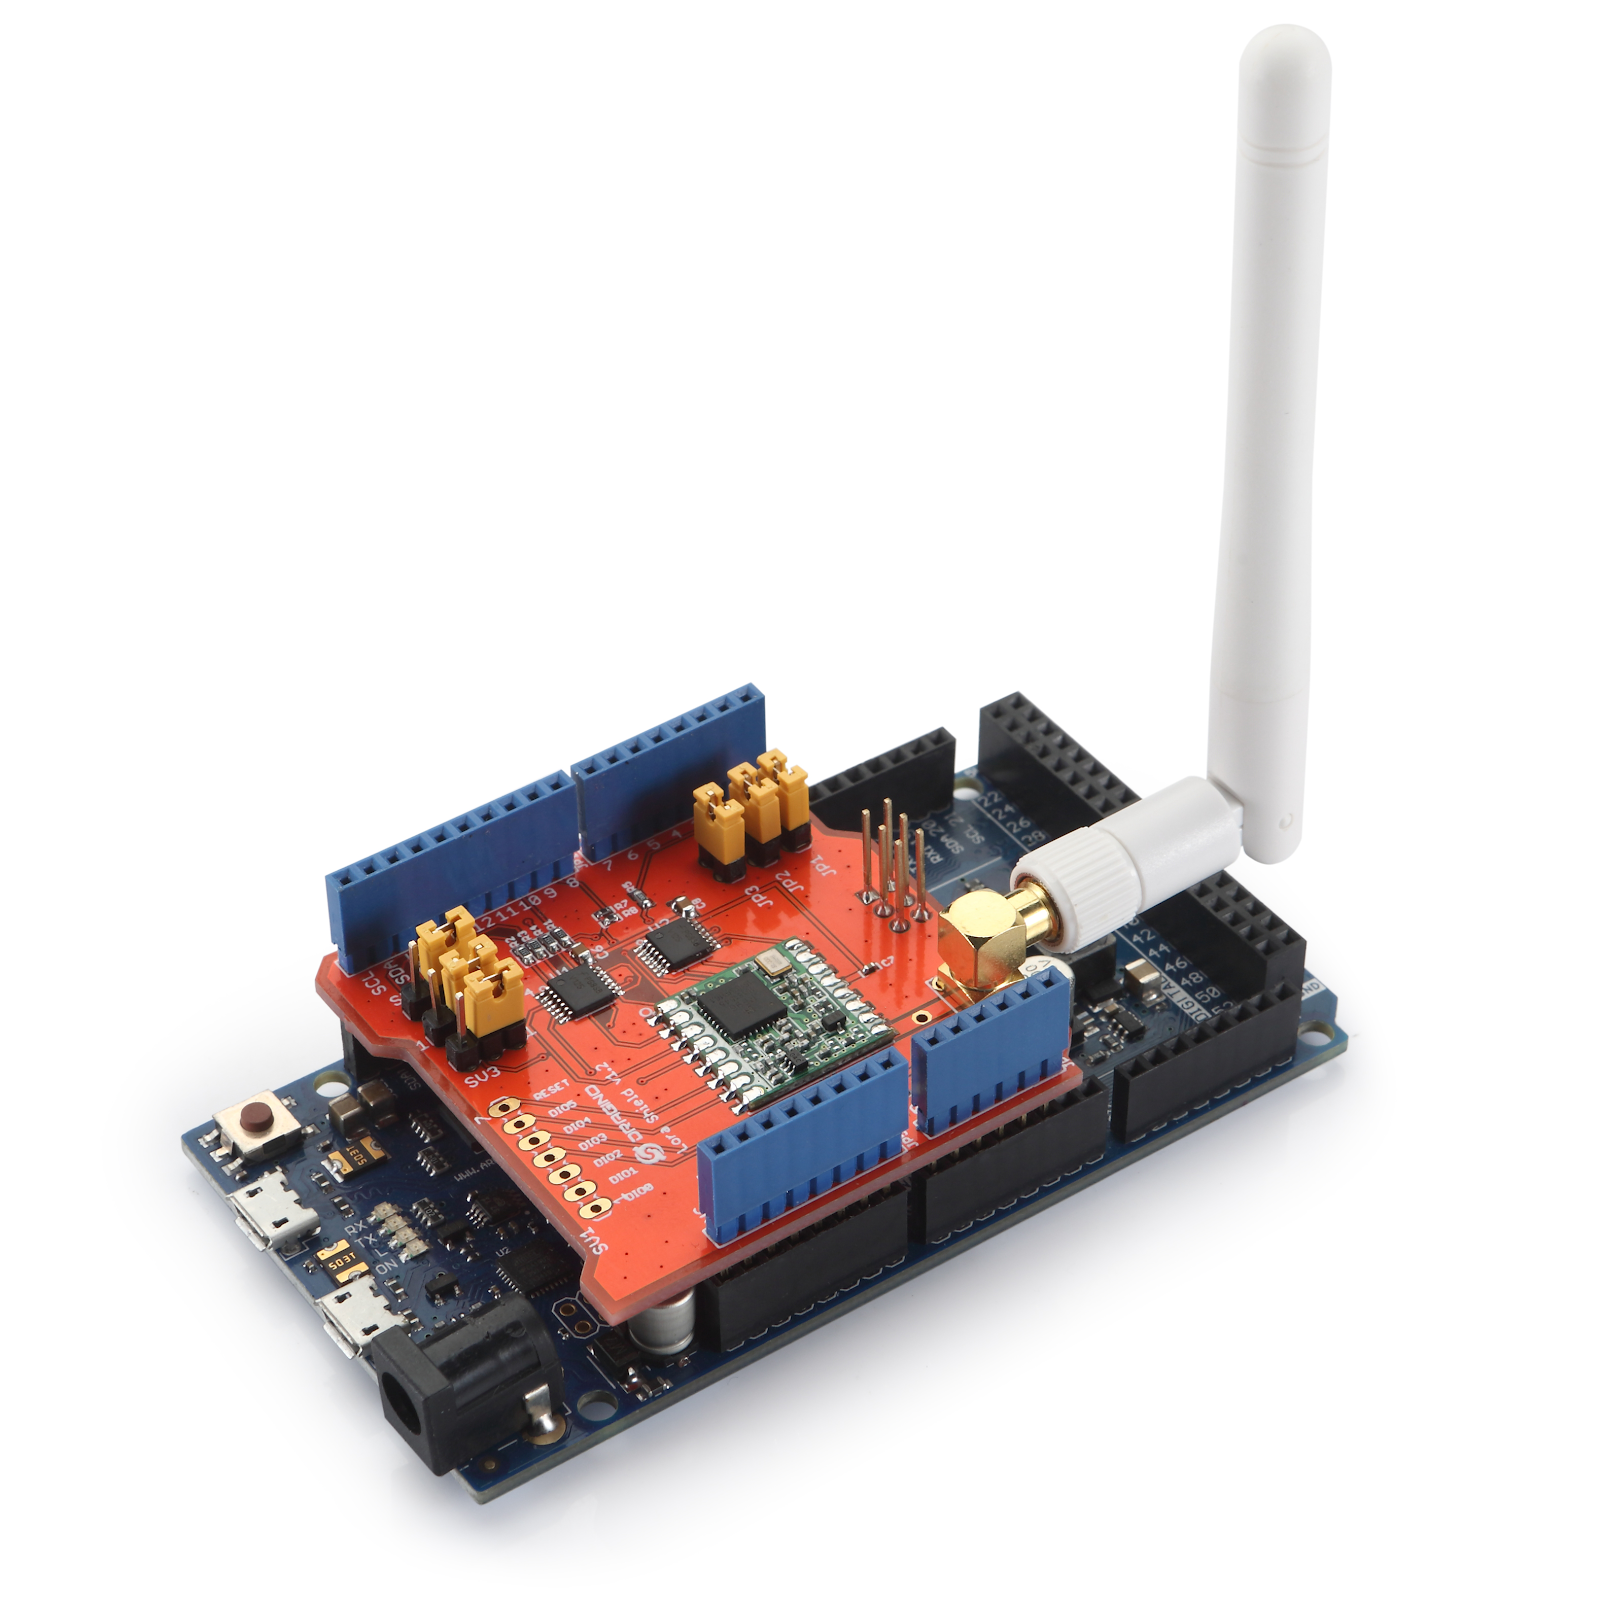
\includegraphics[width=1\textwidth]{figures/arduino.png}
     \caption{Arduino with LoRa shield}
     \label{fig:ard}
    \end{subfigure}%
    \hspace{2em}
    \begin{subfigure}[b]{0.25\textwidth}
     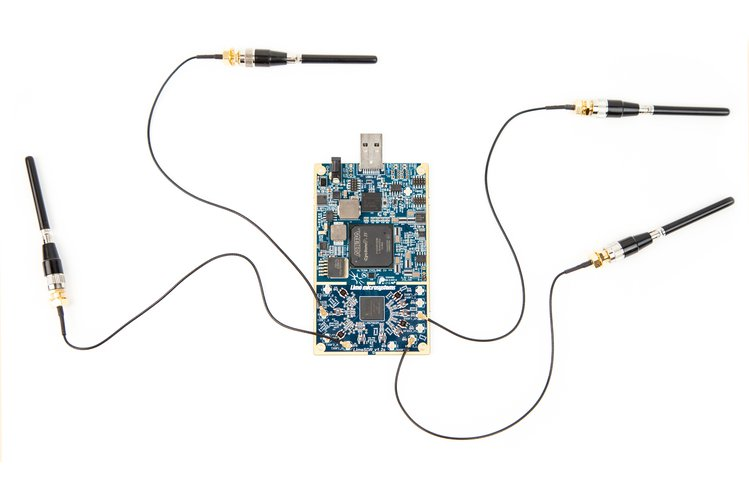
\includegraphics[width=1\textwidth]{figures/limesdr.png}
     \caption{LimeSDR mini}
     \label{fig:sdr}
    \end{subfigure}
    \hspace{2em}
    \begin{subfigure}[b]{0.25\textwidth}
     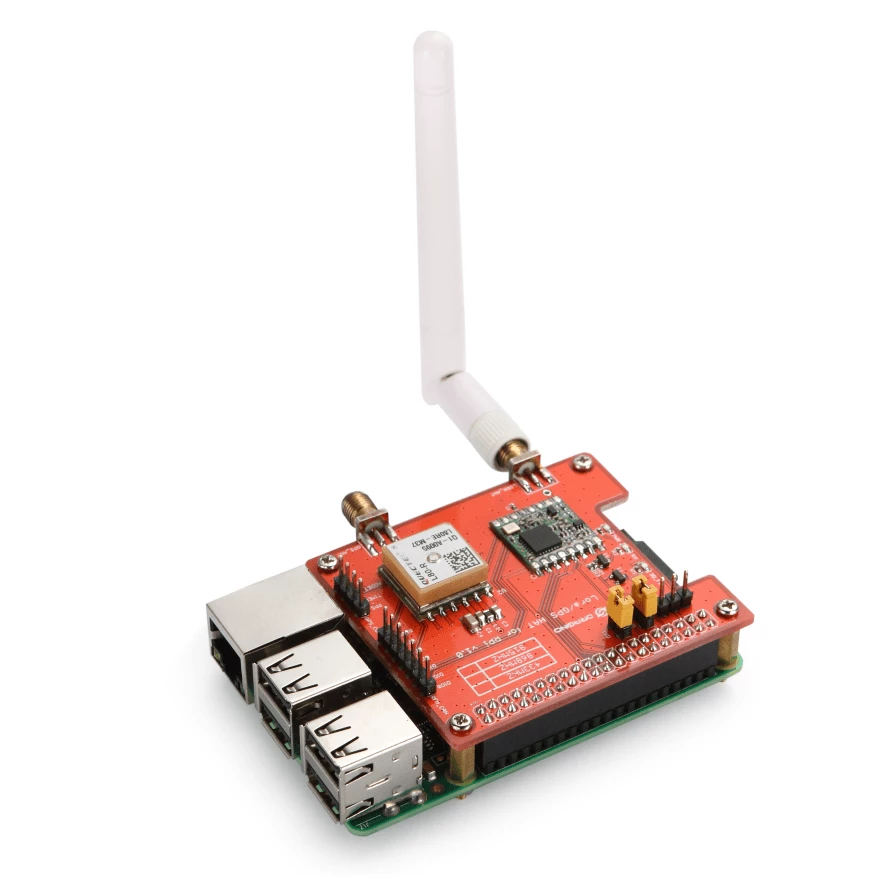
\includegraphics[width=1\textwidth]{figures/raspberry.png}
     \caption{Raspberry Pi with LoRa hat}
     \label{fig:rasp}
    \end{subfigure}
    \caption{Hardware devices}
\end{figure}
% getting a downlink signal
% recording from thethingsnetwrok
% recording from private networks
% manipualting private gateway
% offline generation of downlink signal see chapter

\section{Sending Uplink Signals}
Uplink signals are sent with an arduino device equipped with a LoRa shield. 
The arduino is controlled with an adapted form of the IBM LoraMAC-in-C (LMIC) library, modified to run on arduino devices.
Using this library we implemented a simple communication protocol where a queue of packets is sent out in an interval.
See section~\ref{sec:comm_prot} for detailed information.
% \url{https://github.com/matthijskooijman/arduino-lmic}.

\section{RRH and BBU}
For splitting up the LoRa gateway's functionality we use two laptops. 
One laptop has the LimeSDR mini plugged in and serves as the RRH. The other decodes the LoRa
signal in software, processes the signal and also generates LoRa signals in software and sends those downlink I/Q samples back to the RRH.
The processes on the second laptop run in virtualized environment with docker, more specifically docker compose, dockers orchestration tool.
\\
The LoRa OOT module by Robyns et al. has a branch called "encoder" where they began the implementation of modulating an uplink LoRa signal in software.
It is able to generate a specific test packet but the modulated signal has errors as we saw when we inspected the data payload on the LoRa gateway.
Having an uplink signal generator was a nice starting point, but we needed something to generate downlink signal. In the end we extended the existing implementation
by adding a downlink signal generation ability, see section~\ref{todo}.
\\
Though, as a first workaround we set up a private LoRaWAN network, scheduled a downlink, and recorded it to a file. Now we can stream that file as a response by streaming its content,
which are I/Q samples, to the RRH.


\section{Study Subjects}
\subsection{Network Utilization}
For measuring network traffic, the tool "bmon" is used which stands for bandwidth monitor.
It estimates the bits per second on all available network interfaces, ingoing as well as outgoing. 
\subsection{Impact of Delay}
Speed is essential for most communication systems.
LoRaWAN specifies two receive windows for class A devices. One 1 second after transmission, and if not
received in this window, another one 2 seconds after transmission.
The protocol for this experiment is more lenient. After transmission, the device starts listening
for at least 4 seconds before retransmitting the unacknowledged packet.
\subsection{Network Delay}
Using the command line tool \emph{netem}, which stands for network emulator, we introduce some delay between the RRH and the BBU.
The command is: tc qdisc add dev \emph{interface\_name} root netem delay 200ms. In which \emph{interface\_name} is something like 
eth0. 
\\
This instructs tc (traffic control) to modify the qdisc (queuing discipline) by 
adding (add) a new rule to the device (dev) e.g. eth0 to modify the outbound traffic scheduler (root) using 
the network emulator (netem) with a delay of 200ms~\cite{netem}.
\\
This setup can be easily seen an tested in action:
\begin{itemize}
    \item On the RRH add a delay of 8000ms
    \item On the BBU, in a terminal, type \emph{nc -l 4040}
    \item On the RRH, in a terminal, type \emph{nc <\emph{IP\_ADDRESS\_OF\_THE\_BBU}> 4040}
\end{itemize}

On the RRH on the same terminal on, type a message and send with enter. It should should arrive on the BBU's terminal 
after 8 seconds, which was the case. 

\subsection{Processing Delay}
Not only are network delays of importance, but also the processing time it takes for decoding incoming messages and scheduling downlink messages.
In the python script that sends the downlink, a call to \emph{time.sleep()} can simulate longer processing times.

\section{Architecture}
\subsection{Overview}
This section aims to first give a high level overview of the architecture and then give a more detailed 
architectural overview of each component.
Figure~\ref{fig:high_level_arch} shows the high level architecture with all the hardware components involved.
There are two laptops in the same network connected by an ethernet cable. One laptop serves as an RRH. It has the LimeSDR mini 
plugged into its USB port so it can send and receive signals.
\begin{figure}[h]
    \centering
    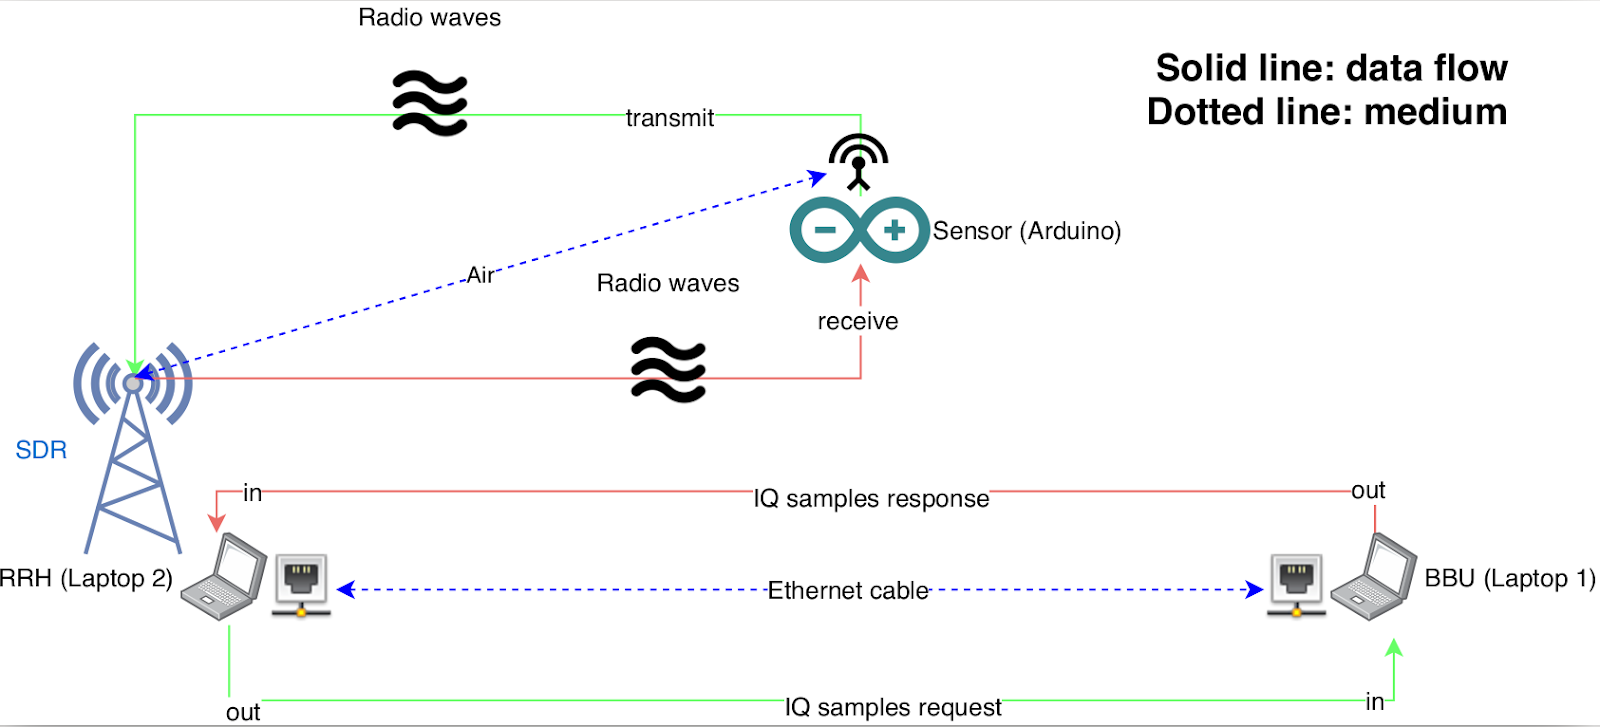
\includegraphics[width=1\textwidth]{figures/high_level_arch.png}
    \caption{High level architecture}
    \label{fig:high_level_arch}
\end{figure}
Incoming signals come from the arduino device. The arduino transmits packets over the air as radio waves. Those get picked up 
by the RRH which converts the analog signal and send them as digital 32bit floats as I/Q samples over ethernet to the second laptop.
This second laptop is the host for the virtual BBU that runs in a docker container. There the signals get demodulated and decoded.
Then the decoded signal gets processed. In case a response is requested, a response signal is generated and sent as I/Q samples back to the RRH.
From the it gets transmitted back to the arduino.
\subsection{Containerization and Orchestration}
Containerization is done with Docker. Docker containers are more lightweight than full virtual machines.
Docker also has a command line tool for container orchestration, called Docker compose. With compose, container configuration is stored in docker-compose.yaml files.
In such a file multiple container configurations can be specified and with a single command i.e docker-compose up, all containers defined in that file start up.
Docker compose also lets the user scale services by spawning new containers on demand.
\subsection{RRH and BBU}
The RRH is the simplest component. It has an antenna for input and one for output. In Figure~\ref{fig:seq_diagram} the RRH is composed by the two 
components "SDR RX" and "SDR TX". They correspond to the physical RX and TX slots ond the SDR device. The BBU is the "Lora Decoder" component. It runs 
in a virtualized environment. Decoded messages get passed to the "Python Script" component. This acts as a network server that schedules an acknowledgement
message back to the arduino. It could run on a third laptop connected via ethernet to the BBU laptop, but for our purposes it runs on the same laptop
as the BBU but in a separate docker container.
\begin{figure}[h]
    \centering
    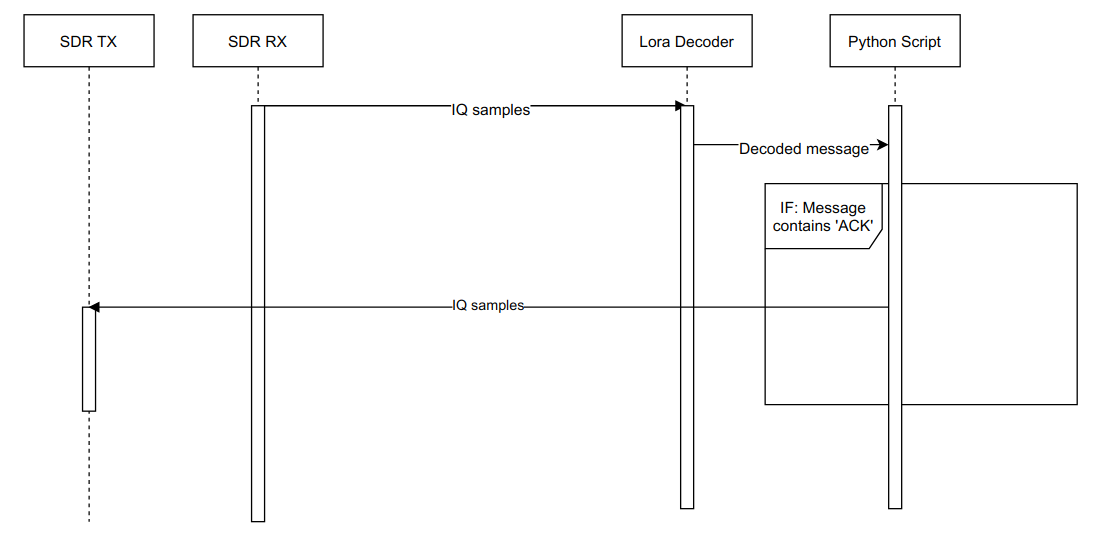
\includegraphics[width=1\textwidth]{figures/seq_diagram.png}
    \caption{Sequence diagram}
    \label{fig:seq_diagram}
\end{figure}


\section{Implementation}
All communication between the components happens over sockets. We use the ZeroMQ (ZMQ) networking library.
It is a good messaging library that offers N-to-N patterns as possible ways to connect the sockets, such as a request-reply pattern
or pub-sub pattern and many more~\cite{zeromq}.
GNU Radio offers ZMQ blocks out of the box, The TCP sink and source blocks for socket communication are still available but deprecated. 
For communication between the RRH and the BBU the pub-sub (publish-subscribe) pattern is used.
Figure~\ref{fig:seq_diagram} shows the "PUB" and "SUB" blocks and the data flow.
The RRH has a PUB sockets that takes as input the I/Q sample stream generated by the RX of the SDR.
The SUB socket in the BBU subscribes to this publishing socket. As this socket connection happens with TCP, the I/Q samples arrive in the order
they are sent an can be directly passed to the LoRa Decoder. Robyns' et al. implementation of LoRa Decoder sends the decoded message 
out on a UDP socket.  The "Python Script" block which is our LoRa network server takes the decoded messages over on this UDP socket and then, streams out 
I/Q samples of the response message over a ZMQ publishing socket to which the RRH's TX slot subscribes to. This closes the cycle.
One of the advantages of using ZMQ is that the sockets can be given the option to not time out or close. This means a subscribing socket 
can be started before a publishing socket without issues. The subscribing socket can wait for the publishing socket to get instantiated. For our architecture 
this means the docker containers for the RRH and BBU can be started in any order and more instances of the BBU can be added at runtime. The sub-pub pattern 
allows new subscribers and publisher to join.

\begin{figure}[h]
    \centering
    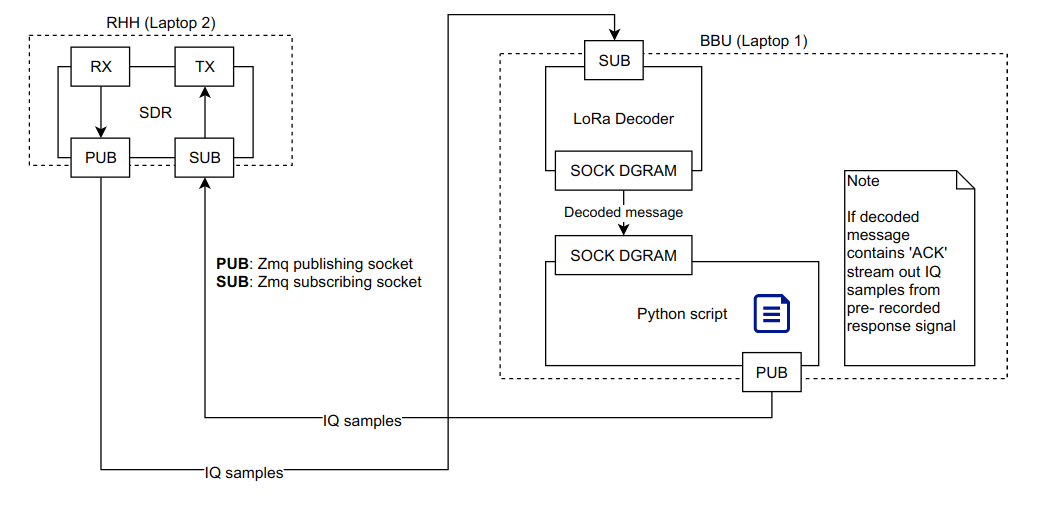
\includegraphics[width=1\textwidth]{figures/impl_diagram.png}
    \caption{Socket communication between components}
    \label{fig:impl_diagram}
\end{figure}

\subsection{RRH}
The RRH implementation is straightforward. Figure~\ref{fig:RRH_impl} show the necessary 
GNU Radio blocks. On the left is the RX block of the LimeSDR that streams the incoming signals to the 
PUB socket. The response message from the networks server to send out comes through a SUB socket which 
streams directly to the TX block of the LimeSDR on the far right of the Figure.
The parameter blocks allow the passing of command line arguments to the resulting application to configure
the socket addresses if necessary. As there is a OOT module needed for GNU Radio to work with the LimeSDR, a the 
RRH comes also in a docker container to quickly get started as the necessary dependencies have all been installed
in that container.
\begin{figure}[h]
    \centering
    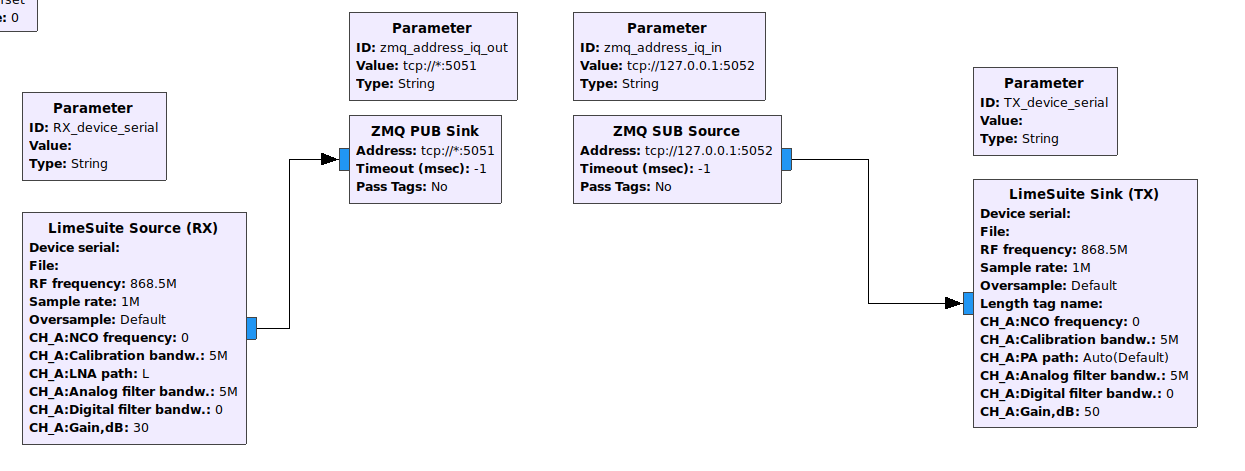
\includegraphics[width=1\textwidth]{figures/RRH_impl.png}
    \caption{GNU Radio blocks for the RRH}
    \label{fig:RRH_impl}
\end{figure}

\subsection{BBU}
The BBU as shown in Figure~\ref{fig:BBU_impl} takes in the RX stream of the RRH on a SUB socket,
passes the I/Q samples to the LoRa decoder. The decoder decodes LoRa signal and outputs them as a 
message on the message socket sink, far right in the Figure.


\begin{figure}[h]
    \centering
    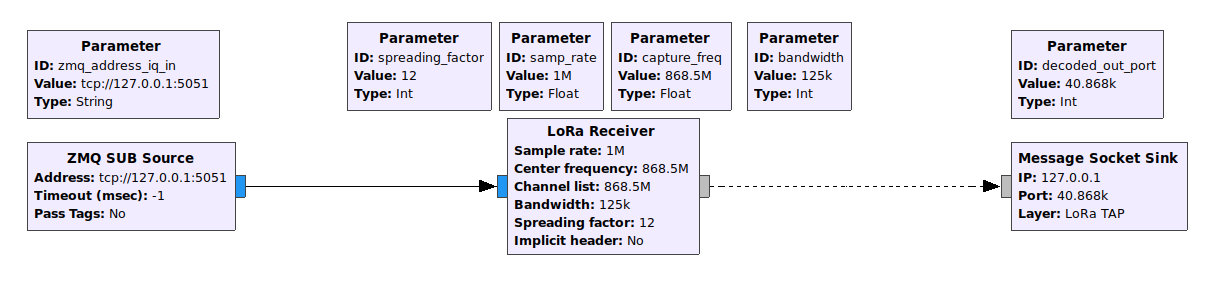
\includegraphics[width=1\textwidth]{figures/BBU_impl.png}
    \caption{GNU Radio blocks for the BBU}
    \label{fig:BBU_impl}
\end{figure}

The python script which acts as our network server, inspects the message payload and if an 
acknowledgement is required by the sender it generates the response signal. 
Listing~\ref{lst:python_code} shows an excerpt of that python script.
The acknowledgement message is a recording of a LoRa downlink signal. Its I/Q samples get read into memory.
The script connects to the UDP socket. As the BBU component and this python script run on the same host, it connects
to 127.0.0.1, the port is passed as argument to the script. As the focus lies on the split between RRH and BBU we decided
to hard code the IP address to localhost for the LoRa decoder and the network server as they run on the same machine as depicted 
in Figure~\ref{fig:impl_diagram}. 
Then, in an endless loop, data gets received from the socket. The buffer size is 1024 bytes.
Whenever "ACK" is in the message payload, the acknowledgement signal get streamed out over a ZMQ publishing socket.
\\
The BBU and the network server run each in a container started with docker compose.


\begin{listing}[h]
\begin{minted}[frame=single,linenos=false]{python}
import zmq
import socket
...
with open (dir_path + "/ACK_DOWN_SF12_CR4.raw") as f:
    ack = f.read()
...
zmq_socket = context.socket(zmq.PUB)
...
s = socket.socket(socket.AF_INET, socket.SOCK_DGRAM)
s.bind(("127.0.0.1", udp_port))
print ('listen for decoded lora packages on udp port ' + str(udp_port))
while True:
    data, addr = s.recvfrom(1024)

    if ("ACK" in data):
        zmq_socket.send(ack) 
    else:
        print ("received package requests no ACK")
     
    
    \end{minted}
    \caption{Excerpt of the python script that functions as the network server}
    \label{lst:python_code}
\end{listing}

\subsection{Communication Protocol Arduino}
\label{sec:comm_prot}

The LMIC library runs a loop that executes jobs scheduled to run at a specified time. 
In the \emph{setup()} function that runs once when the arduino starts settings such as 
the spreading factor, frequency and coding rate are set. The frequency is given in Hertz and the the datarate 
is set with a predefined enum from the LMIC library. Also, the initial job for the LMIC is initialized there, see 
Listing~\ref{lst::ard_setup} last line.

\begin{listing}[h]
    \begin{minted}[frame=single]{c++}
void setup() {
  Serial.begin(9600);
  ...
  // initialize runtime env
  os_init();
  ...
  
  LMIC.freq = 868500000;
  LMIC.txpow = 27; // Maximum TX power
  LMIC.datarate = DR_SF9;
  // This sets CR 4/5, BW125 (except for DR_SF7B, which uses BW250)
  LMIC.rps = updr2rps(LMIC.datarate);

  Serial.println("Started");
  Serial.flush();

  // setup initial job
  os_setCallback(&txjob, my_tx_func);
}
    \end{minted}
    \caption{Arduino setup() function}
    \label{lst::ard_setup}
    
\end{listing}

The last line schedules the initial job  \emph{txjob} with the \emph{my\_tx\_func} function that gets run
on execution of the job, see~Listing~\ref{lst::ard_mytx}. It takes the the index of the packet to send, Listing~\ref{lst::packets}, and
checks if the packet has "ACK" appended. Then the transmit function \emph{tx(packet, callback)} gets executed. 
It takes a packet and a callback function that gets executed after the transmission is finished. 
If an "ACK" is present, the callback function is set to \emph{my\_txdone\_func}, if not it is set to \emph{my\_txdone\_no\_ack\_func}.
Finally, in line 16 in Listing\ref{lst::ard_mytx}, schedules itself to be run again after \emph{TX\_INTERVAL} which is 4 seconds.


\begin{listing}[h]
    \begin{minted}[frame=single]{c++}
#define TX_INTERVAL 4000

int currentPacketIndex = 0;
const int numOfPackets = 3;
char *myPackets[numOfPackets] = {
    "This is packet 1ACK", 
    "This is packet 2ACK", 
    "This is packet 3",
};
    \end{minted}
    \caption{Packets 1 and 2 have "ACK" appended in their payload, while packet 3 does not}
    \label{lst::packets}
    
\end{listing}


\begin{listing}[h]
    \begin{minted}[frame=single, linenos]{c++}
static void my_tx_func(osjob_t *job) {
if (currentPacketIndex < numOfPackets) {
    ...
    char lastThree[3];
    memcpy(lastThree, &myPackets[currentPacketIndex][length - 3], 3);
    const char ack[] = {'A', 'C', 'K'};
    if (!memcmp(lastThree, ack, 3)) {
        // send and start rx for receiving ACK
        Serial.print("transmitting packet with ACK, packet: ");
        tx(myPackets[currentPacketIndex], my_txdone_func);
    } else {
        // send and schedule next packet
        Serial.print("transmitting packet without ACK, packet: ");
        tx(myPackets[currentPacketIndex], my_txdone_no_ack_func);
    }
    os_setTimedCallback(&txjob, os_getTime() +
                            ms2osticks(TX_INTERVAL), my_tx_func);
    } else {
        Serial.println("No more packets to send, done");
    }
}
    \end{minted}
    \caption{\emph{my\_tx\_fun} function}
    \label{lst::ard_mytx}
\end{listing}

The difference between the callback functions passed to the transmission function is that one
waits to receive an acknowledgement while the other simply increases the \emph{currentPacketIndex}
so the next packet gets sent the next time \emph{my\_tx\_func} get called.
The callback to the RX function gets executed every time a packets is received.
Listing~\ref{lst::ard_myrx} shows the implementation. The response signal by sent
by the network server has the payload "ACK", which is three bytes. 
If the \emph{LMIC.dataLen} is three bytes, it is assumed it is the expected acknowledgement signal.
The \emph{currentPacketIndex} gets incremented and the next transmission job gets set up.
Else, the \emph{currentPacketIndex} does not get incremented so the same packet gets rescheduled 
for transmission and the RX function gets called again.


\begin{listing}[h]
    \begin{minted}[frame=single, linenos]{c++}
static void my_rx_func(osjob_t *job)
{
    if (LMIC.dataLen == 3)
    {
    Serial.println("Got ACK");
    // if we get our ACK, start with next transmission, 
    // reschedules transmission at half TX_INTERVAL
    currentPacketIndex++;
    os_setTimedCallback(&txjob, os_getTime()
                            + ms2osticks(TX_INTERVAL / 2), my_tx_func);
    }
    else
    {
    Serial.println("NOT AN ACK");
    // resend packet if no ACK received within 3*TX_INTERVAL,
    // reschedules transmission in 3* TX_INTERVAL
    os_setTimedCallback(&txjob, os_getTime() 
                            + ms2osticks(3 * TX_INTERVAL), my_tx_func);
    // listen again
    rx(my_rx_func);
    }
}
    \end{minted}
    \caption{RX function that checks for the response or reschedules the packet transmission}
    \label{lst::ard_myrx}
\end{listing}

\section{Results}
\subsection{Network Utilization}
Monitoring the network utilization with bmon yields 
335 bytes per second on the ethernet network interface when idle. Once the C-RAN gets started the network
utilization rises to 8MiB/s (Mebibytes) which are equal to 67’108’864 bits.
Bmon only gives an estimation. The theoretical value can be derived the following way:
\\
\begin{itemize}
    \item The LimeSDR had the sample rate set to 1 million samples per second by default.
    \item The type is of complex type of 32 bit, (I/Q) => 2 x 32 bit, which gives 64 million~bits/s
    \item MTU (Maximum Transmission Unit) on most systems is 1500 bytes.
    \item Overhead for TCP and IP is 20 bytes each => 40 bytes
    \item This gives a MSS (Maximum Segment Size) of 1460 bytes
    \item 64M bits ÷ (1460 bytes×8) = 5479.45 packets needed
    \item Total overhead: 5480 packets x (40 bytes x 8) = 175360 bits
    \item 64’000’000 bits + 1’753’600 bits = 65’753’600 bit/s = 7.8 MiB/s
\end{itemize}

The RRH is constantly sending samples to the BBU. It does not matter if the arduino 
sends 1 signal every 4 seconds or 40 signals per second, the network utilization stays the same
as the sample rate stays the same. The experiment worked without error with the 
10 gigabit ethernet connection, but it did not work over Wi-Fi connection.
The response signal sent from the BBU to the RRH did not arrive on the RRH.
\\
\\
\textbf{Optimization}: The load on the network can be reduced. According to the Nyquist-Shannon sampling theorem~\cite{Shannon1949}
a sufficient sampling rate $f_{s}$ for a signal with bandwidth $B$ is given by:
\begin{center}
    $f_{s} > 2*B$  
\end{center}

The signal bandwidth of the LoRa signal sent with the Arduino is set to 125 kHz. Thus the minimum sampling frequency according to the formula above
is 250'000 samples per second which is a quarter of the previous sample rate of 1 million. This also quarters the network utilization from 8 MiB to 2 MiB, see Table~\ref{tabl:samprates}.
Lowering the sampling rate below the Nyquist-Shannon limit results in the signal not getting successfully decoded.
With the sample rate of 125'000 the maximum allowed signal bandwidth to reconstruct that signal is 62.5 kHz so the Arduino signal with 125 kHz bandwidth 
cannot get decoded, see last line in the Table.

\begin{table}[h]
    \centering
    \setlength{\tabcolsep}{22pt}
    \renewcommand{\arraystretch}{1.2}
    \begin{tabular}{cccc}
        \toprule
        Samples & Max. Signal & Network & Decode Success \\
        per second & Bandwidth & Utilization & in Experiment\\
        \midrule
        1'000'000  &500 kHz & 8 MiB/s    &yes\\
        500'000  &250 kHz & 4 MiB/s    &yes\\
        250'000&  125 kHz&  2 MiB/s  & yes\\
        125'000 & 62.5 kHz & 1 MiB/s & no\\
        \bottomrule
       \end{tabular}
\caption{Sampling rates and network utilization}
\label{tabl:samprates}
\end{table}

LoRaWAN defines different regional parameters. In the EU SF 8 to SF 12 signals are sent with 125 kHz bandwidth, while SF 7
can be sent with 125 kHz or 250 kHz bandwidth. In the US on the other hand SF 7 to SF 12 can also be sent with
a 500 kHz bandwidth \cite{lora_wan_reg_params}.
This has to be taken into consideration when designing a LoRaWAN compliant C-RAN architecture.
The network load for decoding a 500 kHz bandwidth US signal is for times higher than a EU 125 kHz bandwidth signal.

\subsection{Cost}
LoRa gateways come in various prices. The low cost indoor commercial gateway by TTN costs around 70\$ while their higher end 
gateway sells for 300\$. Cheaper gateways can be built with and Arduino and a LoRa shield such as the Dragino shield (22\$).
The issue is that those are often based on the SX1272/SX1276 chips. While cheaper, those gateways are so called single channel 
gateways. They can only listen on one channel with one spreading factor. They are not LoRaWAN compliant~\cite{single_chan_gate}.
LoRaWAN compliant gateways can be built with a Raspberry Pi with a iC880A concentrator (130\$) which use the SX1301/SX1257 chips. They can receive packets
of sent with different spreading factors on up to 8 channels in parallel.
\\
The LoRa Decoder block of Robyns et al. does not yet support multichannel decoding. Spreading factor and center frequency
need to be set explicitly, making it a single channel gateway. The advantage of having a decoder in software is that new instances 
of the LoRa Decoder block can be added without additional hardware costs. As the BBU is containerized, starting up a new instance 
is as easy as instructing docker to start a new instance of the decoder and pass it the desired frequency and SF. This saves the costs of 
a LoRaWAN concentrator.
These savings are offset by the need for general purpose hardware the containers can run on and the higher bandwidth requirements.

Using the amazon aws cost calculator \url{https://calculator.s3.amazonaws.com/index.html} the following three fields are of importance : 
\begin{itemize}
    \item Compute:
    \begin{itemize}
        \item  Amazon EC2 Instance
    \end{itemize}
    \item  Data Transfer:
    \begin{itemize}
        \item Data Transfer In
        \item Data Transfer Out  
    \end{itemize}
\end{itemize}

For the EC2 instance we select the \emph{a1.medium} which comes with 1 vCPU and 2 GiB of memory at \emph{0.0255\$} per hour.
\\
\\
Data Transfer In has to be 8 MiB/s to accommodate the maximum possible signal bandwidth of 500 kHz in the US or 
4 MiB/s for the maximal signal bandwidth of 250 kHz in EU. In this cost estimation example we proceed with 4 MiB/s for Europe.
4 MiB per second are 363 GB per day. Data input is free on AWS  giving a daily cost of 0\$.
\\
\\
Data Transfer Out on the other hand does cost. The amount of data that gets sent out depends on
how many uplink signals require a downlink signal. In our example a fixed 3 byte payload response is sent.
In LoRaWAN, downlink messages can have variable length, multiple bytes long.
Sticking with our example, the fixed downlink response signal with a payload of 3 bytes (excluding preamble, header and crc ), SF 7 and coding rate 4/5,
yields an I/Q sample stream of 248 kB (including preamble, header and crc) after modulation.
How many downlink signals will the required? That depends on wether the end-node requires a confirmed uplink.
However, there is an upper limit. The EU specifies a 1\% duty cycle for the 868.0 - 868.6 MHz frequency plan~\cite{duty_cycle}.
The downlink signal has an airtime of 25.86 ms. With a duty cycle of 1\% a downlink signal can be sent every 3 seconds.
This means a maximum of 28'800 downlink signals of this type can be sent by one gateway a day.
Data Transfer Out is thus limited to 7 GB a day if duty cycles are respected, $28800 * 248~kB = 7 GB$.
TTN encourages end-devices to not use confirmed uplinks as most gateways are not designed to send an receive
simultaneously. We assume for our experiment that about 30\% of total possible downlink signals need to be sent
which gives a Data Transfer Out of 2.1 GB/day.
\\
\\
Total monthly cost amounts to 24.07\$:
\begin{itemize}
    \item Compute:
    \begin{itemize}
        \item  Amazon EC2 Instance: 18.67\$
    \end{itemize}
    \item  Data Transfer:
    \begin{itemize}
        \item Data Transfer In: 0\$
        \item Data Transfer Out: 5.40\$  
    \end{itemize}
\end{itemize}

As the modulated signals have to ben sent out over TCP/IP from the BBU to the RRH, a TCP/IP overhead 
of 2.7\% could theoretically be added, but it is negligible as it is an estimation for 
comparison and not for absolute numbers.
\\
\\
In the traditional LoRa setup where the gateway is not split into and RRH and BBU 
component the decoded packet get sent to the network server and not the I/Q samples.
Assuming the same setup as before, instead of calculating $28800 * 248~kB = 7 GB$, the following
has to be calculated: 

\begin{itemize}
    \item payload size: 3 bytes
    \item header size: 4 bytes
    \item CRC size: 0 bytes, downlink messaged do not have a CRC
\end{itemize}

This yield the following $28800 * 7~Bytes = 0.0002016 GB$, which is an insignificant daily amount for AWS as
it gives already 0\$ as cost estimation before we even apply the 30\% usage assumptions.
Thus, sending the I/Q samples over the internet to the cloud is infinitely more expensive compared to just 
sending the demodulated signal. 
\\
However, in a local cloud setup where RRH and BBU are on the same network
or in a network architecture the data does not have to be routed over the internet and 
the BBU can still be virtualized and centralized in a BBU hotel for much cheaper.
In such a setup hardware and operational costs can be saved as outlined in section~\ref{sec:moving_to_cran}.
For each gateway at least 130\$ costs for the LoRa concentrator could be saved by doing its job in software.
For a hobbyist that operates a single gateway it may not be useful as now he needs to invest in general purpose hardware 
that is fast enough to do the decoding in software. Though, for an operator with multiple gateways, centralizing and virtualizing
the decoding has similar benefits as a C-RAN for LTE.

\subsection{Delays}
Various network delays for the outgoing sample stream from the RRH to the BBU were set.
Table~\ref{tabl:delay} summarizes the results.
\\
The higher the delay the less network utilization was measured with bmon. But only after delay,
namely 300ms. Without delay, RX resp. TX on the ethernet ports of the RRH and BBU is 8 MiB/s.
With a 800ms delay it is about 2.32 MiB/s. With a 400 ms delay it is 5.5 MiB/s. With a delay 
of 300ms or less bmon measured still 8 MiB/s.
\\
The expectation was that the signals would get decoded on the BBU the same as without delay just later.
However this was not the case. There was a difference between only a single signal being picked up by the RRH and sent 
to the BBU and the arduino sending multiple signals in an interval and the RRH sending I/Q samples of multiple signals 
to the BBU.
\\
For a delay of 500 ms and below the following held true in the experiment:
\\
\begin{itemize}
    \item The arduino sends a single signal then stops. The RRH receives the signal and sends the I/Q sample stream
    to the BBU. On the BBU the signal gets successfully decoded with a delay of 2 to 10 times the delay set with Netem.
    \item The arduino sends signals in a 4 second interval. The signals get decoded in order on the BBU.
\end{itemize}


For a delay of 500 ms and up the following held true in the experiment:
\\
\begin{itemize}
    \item The arduino sends a single signal then stops. The RRH receives the signal and sends the I/Q sample stream 
    to the BBU. On the BBU the signal does not get decoded.
    \item The arduino send signals in a 4 second interval. Some signals get decoded after the delay times 10. Some signals do not get decoded.
    In an experiment with 800 ms delay,  the first three signals did not get decoded, the fourth signal did after a 10 seconds delay. \\
    Generally, the first signals never got decoded, only the 4th or later signals got eventually decoded by the BBU.
    A possible cause could be that either the LorRa decoder block or the GNU Radio scheduler have an issue 
    with some sort of buffer not being filled fast enough when a single signal is sent and if multiple signals are sent 
    the buffer has time to fill up which leads to some decode success when multiple signals are sent in an interval.
    This is but pure speculation and would need to be investigated further.

\end{itemize}


\begin{table}[h]
    \centering
    \setlength{\tabcolsep}{22pt}
    \renewcommand{\arraystretch}{1.2}
    \begin{tabular}{SScc}
        \toprule 
            {\multirow{1}{*}[-2pt]{Netem Delay}} & {\multirow{1}{*}[-2pt]{Network Traffic }} & \multicolumn{2}{c}{Eventual Decode Success}\\ \cmidrule{3-4}
        
            {(ms)}&{(MiB/s)}&Single Signal & Signal Interval \\
            \midrule
            0  & 8  & yes & yes \\
            20  & 8 & yes & yes \\
            50  & 8 & yes & yes \\
            100  & 8 & yes & yes \\
            200  & 8 & yes & yes \\
            300  & 8 & yes & yes \\
            400  & 5.5 & yes & yes \\
            500  & 4.25 & no & yes \\
            600  & 3.6 & no & yes \\
            800  & 2.3 & no & yes \\
            1000  & 1.92 & no & yes \\
            \bottomrule
    \end{tabular}
    \caption{Effect of delay on network traffic on decode process}
    \label{tabl:delay}
\end{table}

\subsection{Processing Delay}
Processing delays on the LoRa network server were straightforward and as expected. 
Sleep is called in the Python script that sends the downlink. If this is more than the 
time the Arduino is set to listen for downlink signals, the downlink is missed.
For LoRaWAN class A devices this is 1 resp. 2 seconds after uplink.\\
In this example the Arduino sends in an interval of 4 seconds which is more than enough time under good conditions.
However if network delay and processign delays occurs, this changes.
With a Netem delay of 400 ms, the decoded message arrives about 3 seconds later, which leaves only 1 second for the downlink to be sent.
Comparing this to LTE where the requirements impose an upper-bound of less than 3 ms
for TX/RX processing~\cite{Nikaein2015}, LoRaWAN, at least for Class A devices, offers much more leeway.


\chapter{LoRa Tools}
\label{chap:lora_tools}
\section{Getting a Downlink signal}
With the Arduino we could generate raw LorRa signal, record them with the SDR and save them to a file for inspection.
However, getting a downlink signal was not that straightforward. 
In this section, three methods of getting a downlink signal are presented that were tried.
The last method is clearly the winner.

\begin{enumerate}
    \item Schedule a downlink over TTN
    \item Manipulate the packet forwarder of and schedule a downlink over TTN
    \item Manipulate the packet forwarder of the gateway in the private LorRa network.
\end{enumerate}

First idea was to connect the gateway to TTN. 
The Arduino LMIC library provides the LoRaWAN implementation for communicating with a LoRaWAN server like TNN.
After setting up the gateway and Arduino for TTN correctly, the gateways is visible in the TTN dashboard as well as 
the messages that the Arduino sends. Then, in the TTN dashboard a downlink can be scheduled for when the next uplink message 
is received. There are two issues with this method. First, the downlink message will be a LoRaWAN packet. That means when a 3 byte message "ACK"
is sent downlink, the actual signal has all the LoRaWAN fields, as shown in~\ref{fig:lora_wan_struct}, and is encrypted with an AES (Advanced Encryption Standard).
The raw LorRa packet thus has then a length of around 20 bytes.\\
Second, the gateway is free so send the downlink on any valid LoRaWAN frequency with any valid SF it deems reasonable. To get the signal on the desired frequency and SF 
multiple downlinks have to be scheduled one has to wait for the network server to cycle to the next frequency for each new downlink. 
\\
\\
Second, to avoid the varying frequencies and SF, the gateway can be manipulated to send exactly what we want by modifying the source code 
and recompiling.
Changes have to bee done to this file: \url{https://github.com/TheThingsNetwork/packet_forwarder/blob/legacy/poly_pkt_fwd/src/poly_pkt_fwd.c}.
Listing~\ref{lst:polypkt} shows the following necessary changes:
\begin{itemize}
    \item Set the frequency to 8685000000 instead of letting the server decide
    \item In any case set the SF to 12
    \item Override the packet size to 3
    \item Copy the desired payload into the downlink packet payload i.e. "ACK"
\end{itemize}

\begin{listing}[h]
    \begin{minted}[frame=single,linenos=false,breaklines]{c++}
void thread_down(void* pic) {
    ...
    //txpkt.freq_hz = (uint32_t)((double)(1.0e6) * json_value_get_number(val));
    txpkt.freq_hz = 868500000;
    ...
    switch (x0) {
            // case  7: txpkt.datarate = DR_LORA_SF7;  break;
            // case  8: txpkt.datarate = DR_LORA_SF8;  break;
            // case  9: txpkt.datarate = DR_LORA_SF9;  break;
            // case 10: txpkt.datarate = DR_LORA_SF10; break;
            // case 11: txpkt.datarate = DR_LORA_SF11; break;
            // case 12: txpkt.datarate = DR_LORA_SF12; break;
            
            case  7: txpkt.datarate =  DR_LORA_SF12;  break;
            case  8: txpkt.datarate =  DR_LORA_SF12;  break;
            case  9: txpkt.datarate =  DR_LORA_SF12;  break;
            case 10: txpkt.datarate =  DR_LORA_SF12; break;
            case 11: txpkt.datarate =  DR_LORA_SF12; break;
            case 12: txpkt.datarate =  DR_LORA_SF12; break;
            ... 
    }
    ...
    // txpkt.size = (uint16_t)json_value_get_number(val);
    txpkt.size = 3
    ... 
    // i = b64_to_bin(str, strlen(str), txpkt.payload, sizeof txpkt.payload);
    memcpy(txpkt.payload, "ACK", 3);
    i = 3;
    ...
           

        \end{minted}
        \caption{Changes to the polypacket forwarder}
        \label{lst:polypkt}
\end{listing}

This already gives significantly more control and convenience than the first approach. Though, there are two other issues that have to be addressed.
First, there is no guarantee that TTN decides to send the downlink over your manipulated gateway. The TTN network server could decide to send the message over another gateway close enough to
your end-device. In this case the downlink message would not get modified.
\\
Second, your gateway is essentially a trap for the other TTN users. If their downlinks get sent over this manipulated gateway, 
the payload their end-devices receive is modified one. The end devices will probably just drop the packet as 
it is not LoRaWAN conform anymore and also not signed with their key. Nevertheless, this modified gateway is a disruptive factor 
to the TTN network thus this approach should be avoided.
\\
\\
The third method methods is to use a private LoRa server with the modified gateway. 
The ChirpStack project, \url{https://www.chirpstack.io/}, provides open source components of the LoRaWAN stack. 
Once installed, the gateway can be configured to forward the packets to this local LoRaWAN server instead of TTN. 
The ChirpStack application server provides a similar web interface to TTN where gateways and devices and application can be registered.
Now downlinks signals can be scheduled like in a TTN dashboard. The difference is that the downlink will always be sent over the modified gateway
as it is the only gateway registered in this local LoRaWAN network.

\section{Generating a Downlink Signal in Software}
Currently, the Python script in the LorRa C-RAN architecture sends a pre recorded downlink signal as a response to the uplink messages.
This signal was obtained the way described above. Ideally, the downlink signal could be generated on demand in software, enabling dynamic 
payload instead of the static pre recorded "ACK" signal.\\
Robyns et al. decoder repository has branch called encoder which would send out a predefined packet (uplink) as many times as the GNU Radio scheduler 
was able to handle. The packet log on the Raspberry Pi gateway showed the incoming messages, but the payload of each subsequent message was different 
than the one before. The branch was in early development. There was most likely and error in the implementation that propagated with each call to GNU Radios schedular.
So we took the code out of the GNU Radio and refactored this OOT module into a single c++ file that can be executed without GNU Radio. It is hereafter referred as encoder.
Instead of streaming the I/Q samples out to the SDR's TX, the encoder simply writes the generated samples to a binary file.
We then provided the file as input source to the SDR to stream out. Now the gateway showed the same payload for every signal received. 
This means the modulation and encoding process is deterministic for a given input and the issue was indeed with how it was implemented in the GNU Radio framework.
\\
The encoder encodes up and down chirps. Full up chirps for preamble, full down chirps for start of frame delimiter and various length up chirps to encode the data.
To get a downlink signal, we added a flag, and a bit of refactoring, that signals the \emph{transmit\_packet} function to flip all down chirps to up chirps and vice versa.
This generated downlink signal then gets successfully received by the Arduino. 

\section{Improving the Encoder \& Chirp Visualization}
Interestingly, the generate uplink signals by the encoder cannot be decoded 
by the LorRa decoder block, but only by real hardware. According to the author, there are some artifacts
at the symbol boundaries for which real hardware can compensate for but the software decoder cannot.
This is explained in issue 48 on GitHub, \url{https://github.com/rpp0/gr-lora/issues/48}.
\\
To visualize the symbol values of the chirps, the LoRa decoder needs to be modified to save the symbol values at each sample to a file. This file can then be the input to 
the Python visualization script.
To make this process easier, we take the LorRa decoder functionality out of the GNU Radio and put it into a single c++ file.
In GNU Radio the GNU Radio scheduler fed a number of input items in each call of the \emph{work()} function to the decoder and the decoder told the scheduler how many output items it produced with the \emph{consume\_each(int number\_of\_items)} function.
The functions \emph{work} and \emph{consume\_each()} are GNU Radio framework functions we needed to emulate. See \url{https://wiki.gnuradio.org/index.php/BlocksCodingGuide#Basic_Block} for a basic example. \\
To achieve this the \emph{work} function was replace with a while loop and the \emph{consume\_each} function with a pointer arithmetics.
Listing~\ref{lst:gnu_sched} shows the relevant code snippets.

\begin{listing}[h]
    \begin{minted}[frame=single,linenos=false,breaklines]{c++}
int main (){
    ...
    file_size = std::experimental::filesystem::file_size(abs_path);
    uintmax_t total_samples = file_size / sizeof(gr_complex);

    char buffer[BUFFER_SIZE];
    std::ifstream fin(abs_path, std::ios::in | std::ios::binary);
    fin.read(buffer, BUFFER_SIZE);
    input = (gr_complex *)buffer;
    while (read_samples < total_samples)
    {
        work(input);
    }

    ...
}

int work (gr_complex *&input){
    ...
    // consume_each(d_samples_per_symbol);
    read_samples = read_samples + d_samples_per_symbol;
    input = input + d_samples_per_symbol;
    ...
}

bool demodulate () {
    ... 
    outfile << std::hex << word << ',' << std::dec << read_samples << std::endl;
    ...
}
        \end{minted}
        \caption{Emulate the GNU Radio schedular}
        \label{lst:gnu_sched}
\end{listing}

In the programs main function the file with the I/Q samples is read into a buffer.
While there are still samples left to read the work function is called.
\\
In the work function all calls to consume\_each are replaced by incrementing the read samples and
moving the pointer forward by how many samples were consumed.\\
Whenever the decoder calls the demodulate function, we print the value and at which sample it occurred to a csv file.\\
This file and the I/Q sample file are the inputs to the visualization script which then produces a spectrogram chart. \\
Figure~\ref{fig:123_ard} shows an uplink signal sent with the Arduino, Figure~\ref{fig:123_enc} the signal generated with the encoder.
In the original implementation the number of bytes to transmit was set to match only the tespacket, we added the implementation of the formula in
~\ref{sec:pkt_structure} to adjust the number of bytes to transmit dynamically.
This fixed the issue that before, the signal from the encoder did not have 18 symbols like the signal from the Arduino.
Now the number of symbols in the with the encoder generated signal corresponds to the number of symbols in the Arudino signal, however 
the symbol values do not.


\begin{figure}[h]
    \centering
    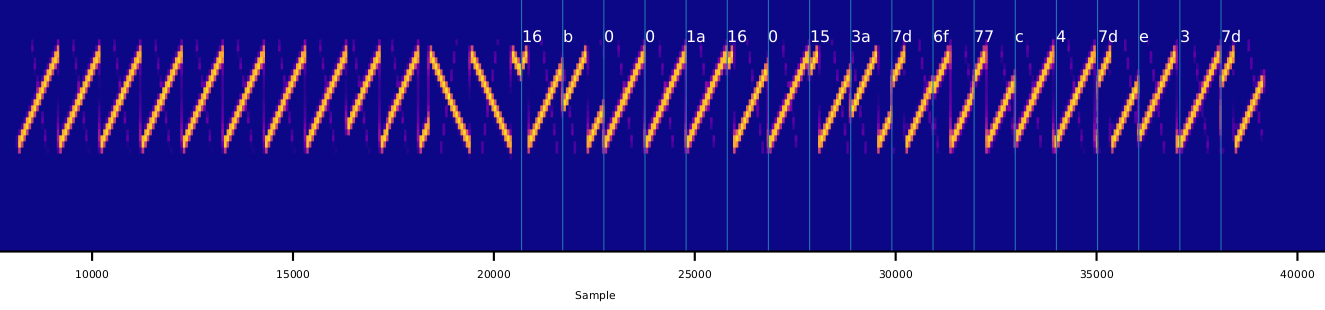
\includegraphics[width=1\textwidth]{figures/123_SF7_CR4_5_arduino.png}
    \caption{123 SF 7, CR 4/5, sent with Arduino}
    \label{fig:123_ard}
\end{figure}

\begin{figure}[h]
    \centering
    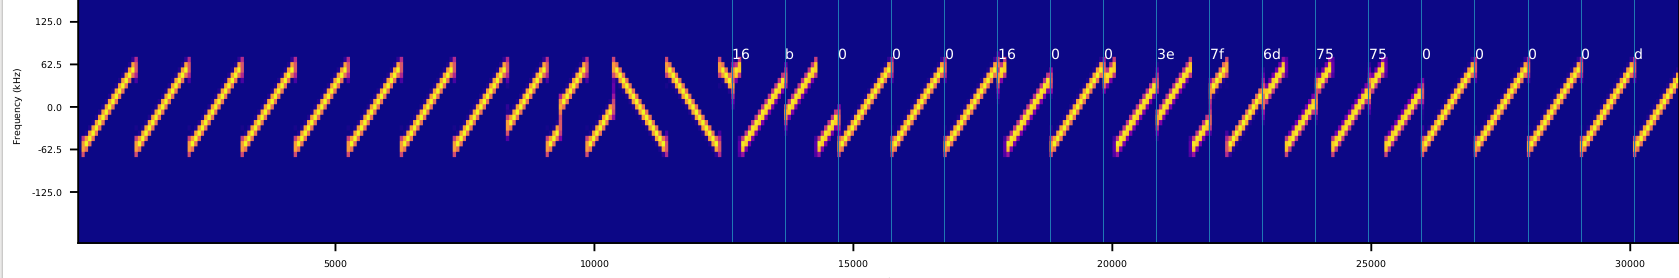
\includegraphics[width=1\textwidth]{figures/123_SF7_CR4_5_from_encode_18_symbols.png}
    \caption{123, SF 7, CR 4/5, sent generated with encoder}
    \label{fig:123_enc}
\end{figure}









